%
\textbf{Chapter 3} %\\
\begin{align*}
\sum_{n\leq x}\tau(n) &= x\log x + (2\gamma-1)x + O(\sqrt x) \\
\sum_{n\leq x}\sigma(n) &= \frac{\pi^2 x^2}{12} + O(x\log x) \\
\sum_{n\leq x}\phi(n) &= \frac{3x^2}{\pi^2} + O(x\log x) \\
\pi(x) &= \sum_{n\leq x}\rho(n) \qquad \rho(n) = \begin{cases}
1 & \text{if $n$ is prime} \\
0 & \text{otherwise}
\end{cases}
\end{align*} \\
\textbf{Chapter 4}
\begin{gather*}
\sum_{n\leq x}\frac{\log p}{p} \\
\sum_{n\leq x}\frac{1}{p} \\
\begin{aligned}
\frac{1}{x}\sum_{n\leq x}\tau(n) &\sim \log x \\
\frac{1}{x}\sum_{n\leq x}\sigma(n) &\sim \frac{\pi^2}{12} x \\
\frac{1}{x}\sum_{n\leq x}\phi(n) &\cong \frac{3}{\pi^2} x
\end{aligned}
\end{gather*}
\eg Find the \# and the \% of lattice points $(a,b)$ visible from $(0,0)$ in the square $\abs{a}$, $\abs{b}\leq x$. \\{}
%[diagram] \\
\[
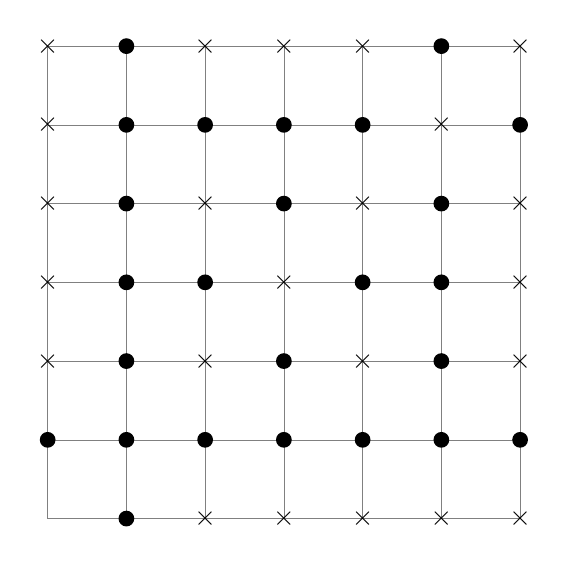
\begin{tikzpicture}
\draw[gray,very thin](0,0) grid (6,6);
\fill(1,0) circle[radius=0.1];
\node at (2,0){$\times$};
\node at (3,0){$\times$};
\node at (4,0){$\times$};
\node at (5,0){$\times$};
\node at (6,0){$\times$};
\fill(0,1) circle[radius=0.1];
\node at (0,2){$\times$};
\node at (0,3){$\times$};
\node at (0,4){$\times$};
\node at (0,5){$\times$};
\node at (0,6){$\times$};
\fill(1,1) circle[radius=0.1];
\fill(2,1) circle[radius=0.1];
\fill(3,1) circle[radius=0.1];
\fill(4,1) circle[radius=0.1];
\fill(5,1) circle[radius=0.1];
\fill(6,1) circle[radius=0.1];
\fill(1,2) circle[radius=0.1];
\fill(1,3) circle[radius=0.1];
\fill(1,4) circle[radius=0.1];
\fill(1,5) circle[radius=0.1];
\fill(1,6) circle[radius=0.1];
\node at (2,2){$\times$};
\node at (3,3){$\times$};
\node at (4,4){$\times$};
\node at (5,5){$\times$};
\node at (6,6){$\times$};
\fill(2,3) circle[radius=0.1];
\fill(3,2) circle[radius=0.1];
\fill(5,2) circle[radius=0.1];
\fill(2,5) circle[radius=0.1];
\node at (2,4){$\times$};
\node at (4,2){$\times$};
\node at (2,6){$\times$};
\node at (6,2){$\times$};
\node at (6,3){$\times$};
\node at (3,6){$\times$};
\node at (6,4){$\times$};
\node at (4,6){$\times$};
\fill(3,4) circle[radius=0.1];
\fill(4,5) circle[radius=0.1];
\fill(4,3) circle[radius=0.1];
\fill(5,4) circle[radius=0.1];
\fill(5,6) circle[radius=0.1];
\fill(6,5) circle[radius=0.1];
\fill(3,5) circle[radius=0.1];
\fill(5,3) circle[radius=0.1];
\end{tikzpicture}
\]
$(a,b)$ is visible when $\gcd(a,b)=1$

The \# of visible points $(k,l)$ with $\abs{a}$, $\abs{b}\leq x$ is
\begin{align*}
8 + 8\sum_{k\geq2}\phi(k) &= 8\sum_{k\geq1}\phi(k) \\
&= 8\paren[\Big]{\frac{3}{\pi^2}x^2+O(x\log x)} \\
&= \frac{24}{\pi^2} x^2 + O(x\log x)
\end{align*}
\# of $(k,l)$ in the square $\abs{k}$, $\abs{l}\leq x$ is
\[ (2\floor{x}+1)^2 = (2x+O(1))^2 = 4x^2 + O(x) \]
The \% of visible points is
\begin{align*}
\frac{\frac{24}{\pi^2}x^2+O(x\log x)}{4x^2+O(x)} &= \frac{\frac{24}{\pi^2}+O(\frac{\log x}{x})}{4+O(\frac1x)} \\
\to\frac{24/\pi^2}{4} &= \frac{6}{\pi^2} \text{ as $x\to\infty$} 
\end{align*}
\textbf{Euler's recursion formula for $\sigma(n)$}
\[ (1-x)(1-x^2)(1-x^3)\dotsm \]
A partition of $n$ into $k$ parts $(a_1,a_2,\dotsc,a_k)$, $1\leq a_1\leq a_2\leq\dotsb\leq a_k$, $\sum a_i=n$ \\
Let $P=\brace{\text{of all partitions (of any $n$ into any \# of parts)}}$ \\
$\operatorname{weight}(a_1,\dotsc,a_k)=\sum a_i$
\begin{align*}
P &= \underset{1+x+x^2+\dotsb}{\brace{\emptyset,1,11,111,\dotsc}} \underset{1+x^2+x^4+\dotsb}{\brace{\emptyset,2,22,222,\dotsc}} \underset{1+x^3+x^6}{\brace{\emptyset,3,33,\dotsc}}, \dotsc \\
\Phi_P &= \frac{1}{1-x} \cdot \frac{1}{1-x^2} \cdot \frac{1}{1-x^3} \dotsm \\
(1-x)(1-x^2)(1-x^3)(1-x^4)\dotsm &= 1 - x^1 - x^2 - x^3 - x^4 - \dotsb \\
&\quad + x^{1+2} + x^{1+3} + x^{1+4} + x^{2+3} + x^{2+4} + x^{3+4} + \dotsb \\
&\quad - x^{1+2+3} - x^{1+2+4} - x^{1+3+4} - x^{2+3+4} - \dotsb \\
&\quad + x^{1+2+3+4} + \dotsb %\\
%&\quad \vdots
\end{align*}
\[ \therefore \prod_{k=1}^\infty (1-x^k) = \sum (c_n x^n) \]
where
\begin{gather*}
\begin{multlined}
c_n=(\text{\# of parititions of $n$ into an even \# of distinct parts})\\
-(\text{\# of partitions of $n$ into an odd \# of distinct parts})
\end{multlined} \\
\begin{matrix}
1 &-x \\
1 &-x &-x^2 &+x^3 \\
&&&-x^3 &+x^4 &+x^5 &-x^6 \\\hline
%1 & -1 & -1 & 0 & 1 & 1 & -1
1 & -1 & -1 & 0 & 0 & 1 & 0 & 1 & 1 & 0 & -1 & -1 & -2 \\
&&&&&&&&                 -1 & 1 & 1 & 0 & 0 \\ \cline{9-13}
&&&&&&&&                  0 & 1 & 0 & -1&-2 \\
&&&&&&&&                    & -1& 1 &  1& 0 \\ \cline{10-13}
&&&&&&&&                    &  0& 1 &0  &-2 \\
&&&&&&&&                    &   & -1& 1 & 1 \\ \cline{11-13}
&&&&&&&&                    &   &  0& 1 &-1 \\
&&&&&&&&                    &   &   & -1& 1 \\ \cline{12-13}
&&&&&&&&                    &   &   &  0& 0 \\
&&&&&&&&                    &   &   &   &-1 \\ \cline{13-13}
&&&&&&&&                    &   &   &   &-1
\end{matrix} \\
\begin{aligned}
\prod(1-x^k) &= \sum c_n x^n \\
&= 1 - x^1 - x^2 + x^5 + x^7 - x^{12} - x^{15} + \quad + \quad - \quad -
\end{aligned}
\end{gather*}
%$1-x$
%$1-x-x^2+x^3$
%$       -x^3+x^4+x^5-x^6$
%1 -1 -1 0 0 1 0 1 1 0 -1 -1 -2
%                 -1 1  1  0  0
%                 -------------
%                  0 1  0 -1 -2
%                   -1  1  1  0
%                   -----------
%                    0  1  0 -2
%                      -1  1  1
%                      --------
%                       0  1 -1
%                         -1  1
%                         -----
%                          0  0
%                            -1
%                            --
%                            -1
%
%\begin{align*}
%\prod(1-x^k) &= \sum c_n x^n \\
%&= 1 - x^1 - x^2 + x^5 + x^7 - x^{12} - x^{15} + \quad + \quad - \quad -
%\end{align*}
$n(3n\pm1)/2$ \\
\conj $=\sum_{n\in\Z}(-1)^n x^{n(3n+1)/2}$ \\
$1-\sum(1-yx)(1-yx^2)(1-yx^3)$ \\
$f(x,y)=\cdots f(xy,y)$

$\sigma(n)$
\begin{align*}
f(x) &= \prod_{k=1}^\infty(1-x^k) \\
\log f(x) &= \sum\log(1-x^k) \\
\frac{f'}{f} &= \sum_{k=1}^\infty \frac{-kx^{k-1}}{1-x^k} = \frac{-1}{1-x} - \frac{2x}{1-x^2} - \frac{3x^2}{1-x^3} - \dotsb \\
-\frac{xf'}{f} &=
\begin{matrix}
1 &+ x &+ x^2 &+ x^3 &+ x^4 &+ x^5 &+ x^6 &+ x^7& &+\dotsb \\
  & +2x &      & +2x^3    &      & +2x^5    &      & +2x^7   & &+\dotsb \\
  &    & +3x^2    &      &      & +3x^5    &      &     &+3x^8 &+\dotsb \\
  &    &      & +4x^3    &      &      &      & +4x^7   & &+\dotsb
\end{matrix} \\
               &= \sum \sigma(n) x^{n-1} \\
f(x) &= 1 - x - x^2 + x^5 + x^7 - x^{12} - x^{15} + \dotsb \\
f' &= -1 -2x + 5x^4 + 7x^6 - 12x^{11} - 15x^{14} + \dotsb \\
\sum\sigma(n)x^{n-1} = -\frac{xf'}{f} &= \frac{-x-2x^2+5x^6+7x^7-12x^{12}-15x^{15}+\dotsb}{1-x-x^2+\dotsb} \\
&= (\sigma(1)+\sigma(2)x+\sigma(3)x^2+\dotsb)(1-x-x^2+x^5+x^7-\dotsb) \\
&= (-1-2x^2+5x^5-7x^7-12x^{12}+\dotsb)
\end{align*}
This gives Euler Recursion Formula

$3+5+6=14$ %\\{}
%[diagram] \\
%...... \\
%..... \\
%...
\begin{center}
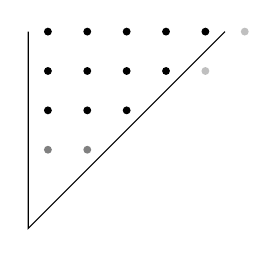
\begin{tikzpicture}[scale=0.5]
\fill(0,3)circle[radius=0.1];\fill(1,3)circle[radius=0.1];\fill(2,3)circle[radius=0.1];\fill(3,3)circle[radius=0.1];\fill(4,3)circle[radius=0.1];\fill[color=lightgray](5,3)circle[radius=0.1];
\fill(0,2)circle[radius=0.1];\fill(1,2)circle[radius=0.1];\fill(2,2)circle[radius=0.1];\fill(3,2)circle[radius=0.1];\fill[color=lightgray](4,2)circle[radius=0.1];
\fill(0,1)circle[radius=0.1];\fill(1,1)circle[radius=0.1];\fill(2,1)circle[radius=0.1];
\fill[color=gray](0,0)circle[radius=0.1];\fill[color=gray](1,0)circle[radius=0.1];
\draw(-0.5,3)--(-0.5,-2)--(4.5,3);
\end{tikzpicture}
\end{center}
